\chapter{Organizacja oprogramowania}
\label{organizacja_opr} 


\section{ESP8266 RTOS SDK}
\label{sdk}
W ramach projektu, za stroną producenta, zdecydowałem się na skorzystanie z 
szkieletu aplikacyjnego \verb+ESP8266_RTOS_SDK+, wykorzystującego FreeRTOS.
Takie podejście pozwala na pisanie prostych aplikacji wielozadaniowych. Dodatkowo, 
szkielet udostępnia rozbudowane API, które znacznie upraszcza korzystania z peryferiali oraz sieci Wi-Fi. 

\subsection{Instalacja środowiska}
\label{instalacja}
Dużą zaletą środowiska \verb+ESP8266_RTOS_SDK+ przygotowanego przez firmę \textit{Espressif}
jest prostota instalcji i korzystania z niego. Środowisko można pobrać ze strony producenta
lub z publicznego repozytorium znajdującego się w serwisie \verb+github.com+. Po instalacji
i ustawieniu koniecznych zmiennych środowiskowych, można przystąpić do wgrania programu.

\subsection{Tworzenie programu}
\label{tworzenie programu}
W celu stworzenia własnego aplikacji na moduł \verb+ESP8266+ należy skopiować folder 
\verb+project_template+ do wybranego folderu i w pliku \verb+user_main.c+ zapisać swój kod
źródłowy. Struktura przykładowego programu została przedstawiona w \ref{example_C}.

\subsection{Kompilacja i wgranie programu}
\label{kompilacja}
Środowisko znacząco upraszcza pracę nad aplikacjami, ponieważ dostarcza plik \verb+Makefile+
który samemu zajmuje się kompilacją i wgrywaniem programu. Z poziomu programisty, należy jedynie
wywołać polecenie \texttt{make flash}, które kolejno wywoła kompilator \verb+xtensa-lx106-elf-gcc+
a następnie narzędzie do wgrywania \verb+esptool.py+ napisane w języku Python.

W przypadku zwykłych modułów, konieczne jest ręczne ustawienie określonych pinów GPIO w taki sposób
aby przy resecie urządzenia przeszło ono w tryb UART, pozwalający programować pamięc Flash.
Po wgraniu programu, należy zresetować urządzenie, tak aby uruchomić bootloader w trybie FLASH, 
pozwalający na normalną pracę urzadzenia. Oprócz tego, istnieje jeszcze tryb SD, umożliwiający 
uruchomienie systemu z karty SD. Sposób ustawienia pinów został przedstawiony w tabeli 
\ref{tabela_trybow}

\begin{table}[H]
    \centering
    \begin{tabular}{lccc}
    \hline
          & \multicolumn{1}{l}{GPIO0} & \multicolumn{1}{l}{GPIO2} & \multicolumn{1}{l}{GPIO15} \\ \hline
    UART  & 0                         & 1                         & 0                          \\
    FLASH & 1                         & 1                         & 0                          \\
    SD    & x                         & x                         & 1                         
    \end{tabular}
    \caption{Porównanie pinów badanych przez bootloader podczas uruchamiania systemu}
    \label{tabela_trybow}
\end{table}
\FloatBarrier
\newpage
W przypadku modułu ESP8266-EVB użyczonego z zasobów Instytutu Informatyki w ramach tego projektu,
producent umieścił na płytce przycisk pozwalający na ustawienie omawianych pinów
w odpowiedni sposób tak aby przy włączeniu urządzenia przy wciśniętym przycisku, wchodził
on w tryb UART.

\begin{figure}[H]
	\centering
    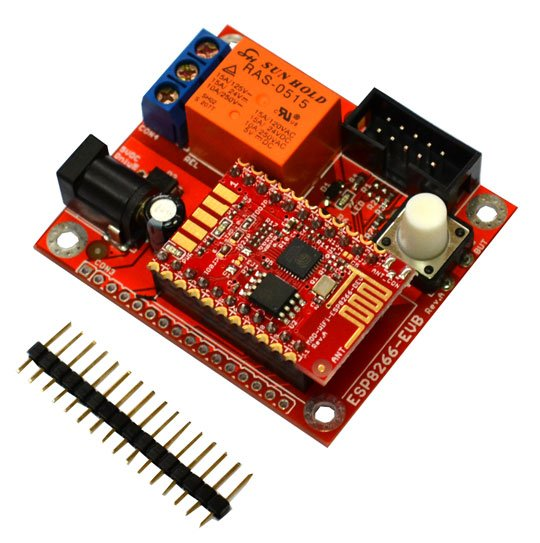
\includegraphics[width=8cm]{./images/ESP8266-EVB.jpg}
    \caption{Płytka ESP8266-EVB firmy OLIMEX}
	\label{esp8266-evb}
\end{figure}
\FloatBarrier

W przypadku finalnie wykorzystanego przeze mnie modułu NodeMCU w wersji 3 z modułem
ESP8266, nie było potrzeby ręcznego przestawiania trybu pracy. Wszystkim tym zajmowało
się program do wgrywania kodu. Znacznie ułatwiało i przyspieszało to pracę nad projektem.
Płytka ta jest zasilana z kabla USB, który podpięty do komputera służył również do komunikacji
przez port szeregowy.

\begin{figure}[H]
	\centering
    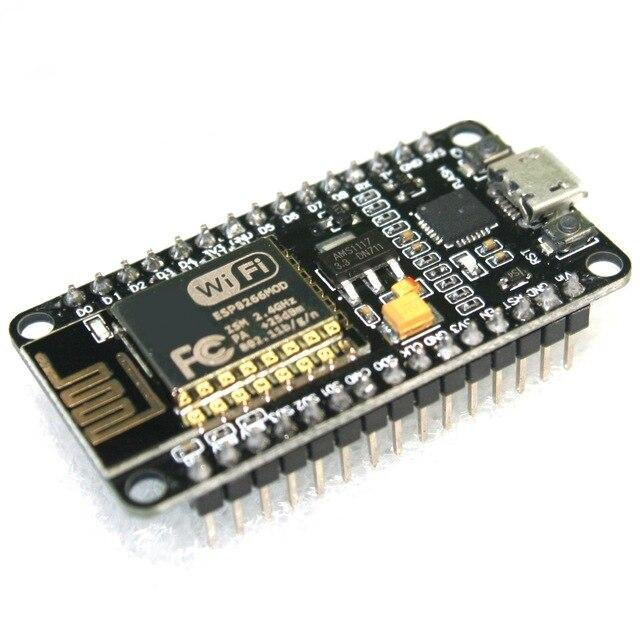
\includegraphics[width=8cm]{./images/nodemcu.jpg}
    \caption{Wykorzystana płytka ewaluacyjna NodeMCU v3}
	\label{esp8266-nodemcu}
\end{figure}
\FloatBarrier

\subsection{Narzędzie \texttt{esptool.py}}
\label{esptool}
Narzędzie \texttt{esptool.py} umożliwia prgoramowanie modułu ESP8266. Zostało one 
napisane w języku Python w wersji 2. Aby zaprogramować płytkę należy wywołać 
program z odpowiednimi argumentami. Przykładowa komenda wygląda w następujący sposób:

\begin{lstlisting}[style=customc,
    frame=single,
    caption={Przykładowa komenda programująca moduł ESP8266},
    captionpos=b,
    label={esptool_basic}]
esptool.py --port COM4 write_flash 0x1000 my_app-0x01000.bin
\end{lstlisting}

Po komendzie \texttt{write\_{}flash} należy zapisać adres początkowy programu w 
pamięci Flash. Program umożliwia również konwersję plików \texttt{.elf} do postaci 
binarnej \texttt{.bin}. 

\texttt{esptool.py} pozwala również załadować program do pamięci RAM, tak jak to było
wspomniane w \ref{pamiec}. Aby w ten sposób wgrać program, należy skorzystać z polecenia 
\texttt{load\_{}ram}.

\section{Budowa przykładowego programu w języku C}
\label{example_C}

